
Programmet kan køres via den udleverede .jar-fil med følgende kommando ``java -jar -Xmx2G map.jar''. Når programmet er startet op, skal man vælge hvilket data-sæt man vil benytte.

\begin{figure}
\centering
\begin{minipage}{.5\textwidth}
  \centering
	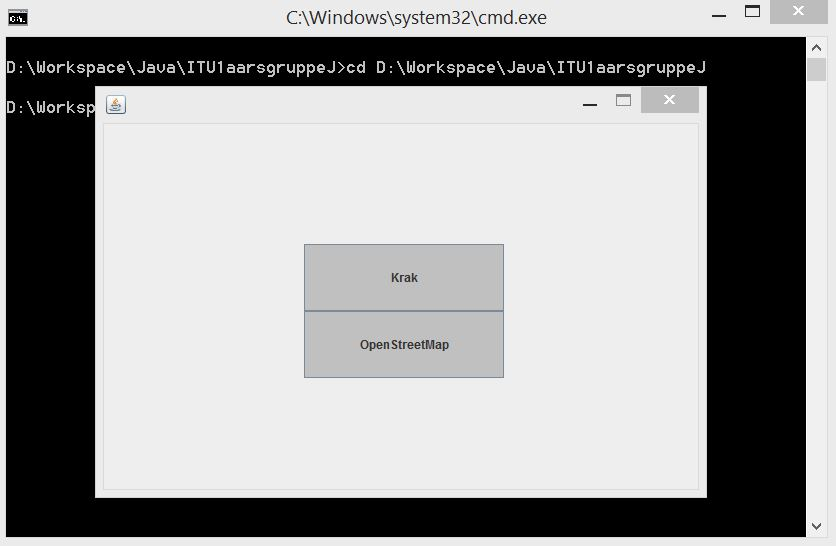
\includegraphics[width=(0.95\textwidth)]{brugervejledning/vaelgdata}
  \end{minipage}%
\begin{minipage}{.5\textwidth}
  \centering
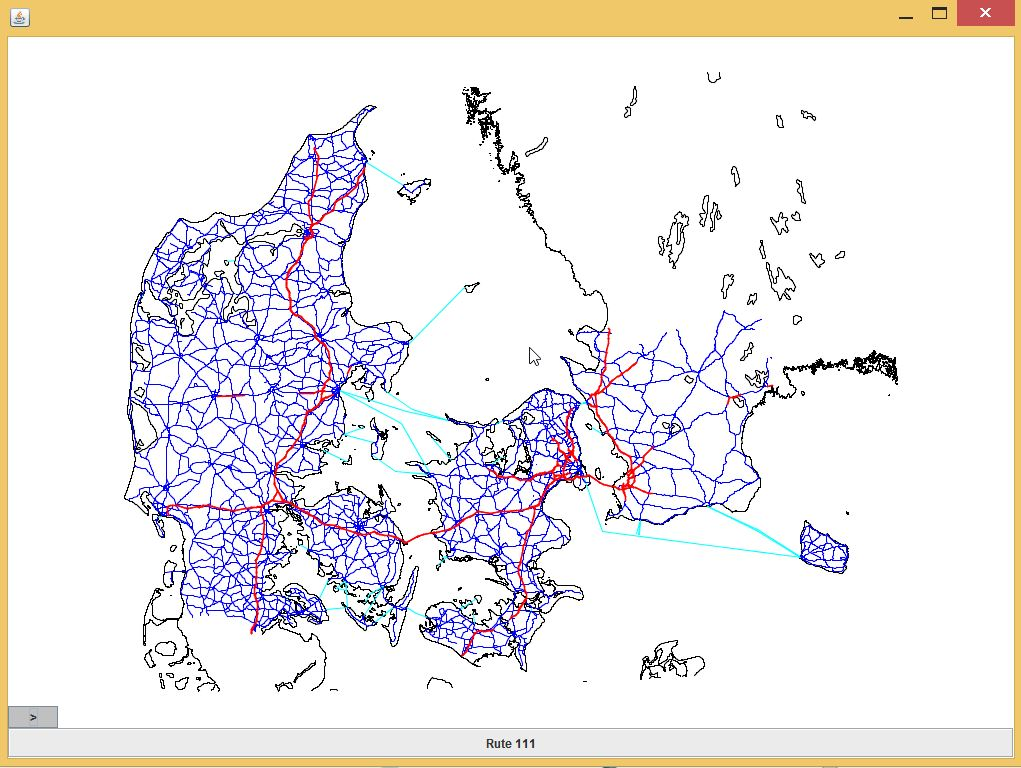
\includegraphics[width=(0.95\textwidth)]{brugervejledning/renkort}
\end{minipage}
\end{figure}


\subsection{Kortmanipulation}

\begin{table}[h!t]
\centering
	\caption{Tastaturgenveje}
	\begin{tabular}{p{6cm} l l l}
		\hline\hline
		Kommando & Tast & Tast & Tast \\ [0.5ex]
		\hline
		Zoom kortet ind & i & + & num+\\
		Zoom kortet ud & o & - & num-\\
		Returner til startzoomgrad og centrer kortet & r & backspace\\
		Bevæg kortet & piletasterne\\
		Vis/skjul rutevejledningsmenu & space \\
		\hline
	\end{tabular}
\end{table}

\begin{table}[h!t]
\centering
	\caption{Mussemanipulation}
	\begin{tabular}{p{6cm} l l p{4cm}}
		\hline\hline
		Kommando & bruger \\ [0.5ex]
		\hline
		Zoom kortet ind & Rul musehjulet væk fra bruger\\
		Zoom kortet ud & Rul musehjulet hen mod bruger\\
		Zoom kortet ind i markeret område & Højreklik, træk og slip så du har det ønskede udsnit\\
		Returner kortet til startzoomgrad og centrer kortet & Tryk på den midterste museknap\\
		Bevæg kortet & Venstreklik, træk og slip så du har det ønskede udsnit\\
		åbn/luk rutevejledningsmenu & benyt knappen nede i venstre hjørne\\
		\hline
	\end{tabular}
\end{table}

\subsection{Rutevejledning}

Man kan enten benytte musen på kortet for at få en rutevejledning, eller man kan benytte sidebaren. Man benytter musen ved at højreklikke på sin start position, og så klikke med venstre musetast på sin slutdestination. I tilfælde af at man benytter sidebaren, skriver man udgangspunktets destination i felt (A) og destinationens adresse i felt (B), hvorefter man trykker på knappen: ``Get route''. Der vil nu vises en rutevejledning i sidebaren, såvel som at ruten vil være tegnet med en magenta farve på kortet.

\begin{figure}
\centering
\begin{minipage}{.5\textwidth}
  \centering
	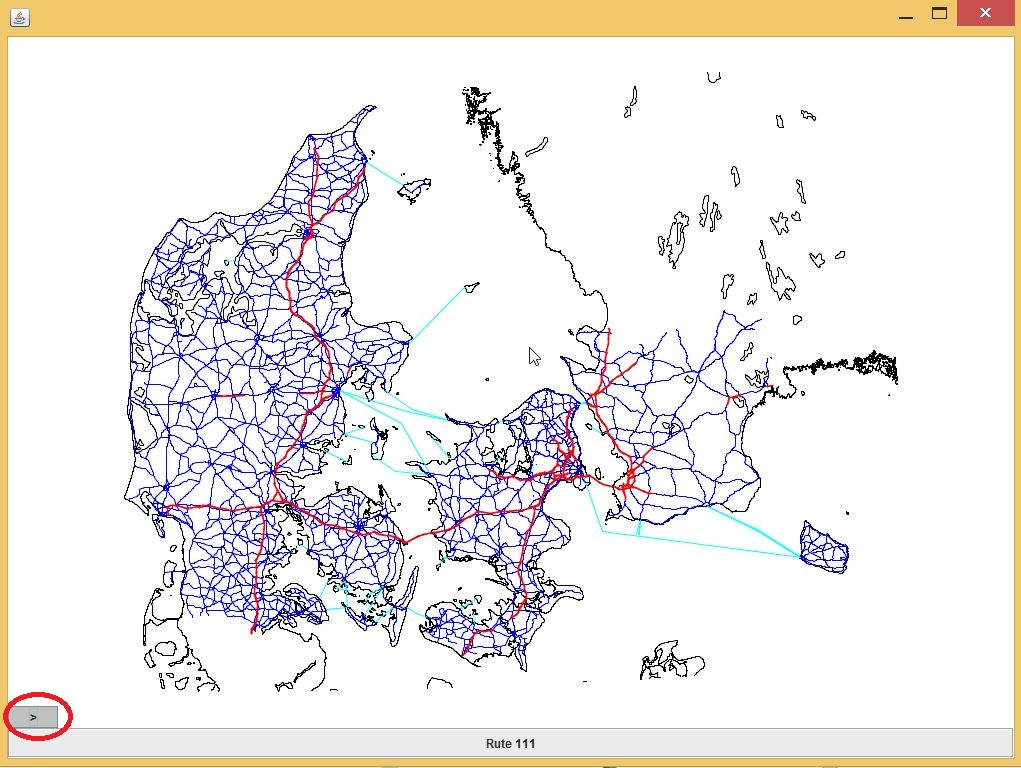
\includegraphics[width=(0.95\textwidth)]{brugervejledning/halvrenkort}
  \end{minipage}%
\begin{minipage}{.5\textwidth}
  \centering
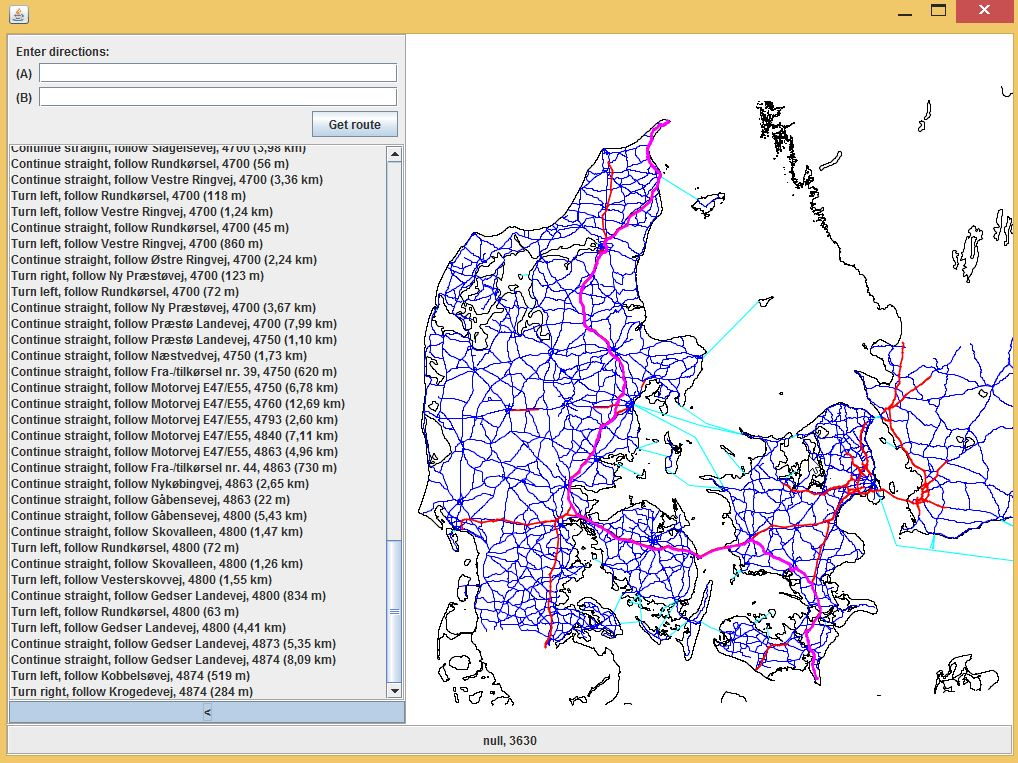
\includegraphics[width=(0.95\textwidth)]{brugervejledning/klikkort}
\end{minipage}
\end{figure}
